\begin{frame}{Statistics on Human Effort}

\begin{itemize}
    \item Manual evaluation done by:-
    \begin{itemize}
        \item shared task participant
        \item interested volunteers
        \item small number of paid of annotators
    \end{itemize}
\end{itemize}

\vfill

\begin{block}{Participation Statistics}
\begin{itemize}
    \item More than 160 people participated, with 100 people putting more than an hours worth of work, and 30 putting more than 4 hours.
    \item collectively 479 hours was spent.
\end{itemize}
\end{block}

\end{frame}


\begin{frame}{Overview of Evaluation Strategy}

\begin{block}{Core Philosophy}
Automatic metrics are imperfect, greater emphasis on human judgment 
\end{block}

\vfill

\begin{block}{Three Primary Tasks}
\begin{itemize}
    \item Sentence Ranking: The official determinant of system quality.
    \item Editing MT Output: Assessing fluency and intelligibility.
    \item Acceptability Judging: Verifying the correctness of edited output.
\end{itemize}
\end{block}

\end{frame}


\begin{frame}{Task 1 --- Sentence Ranking}

\begin{block}{The Official Metric}
\begin{itemize}
    \item The Process: Annotators are shown a source sentence and up to 5 system translations.
    \item The Instruction: "Rank translations from Best to Worst (ties allowed)."
    \item Scoring: Systems are ranked based on how frequently they are judged "better than or equal to" others.
\end{itemize}
\end{block}

\vfill

\begin{block}{Scale}
Over 35,000 individual rankings were collected across all language pairs
\end{block}

\end{frame}


\begin{frame}{Task 2 --- Editing MT Output}

\begin{block}{Measuring Fluency and Intelligibility}
\begin{itemize}
    \item Experimental Design: Judges see MT output without the source or reference translation.
    \item The Task: Edit the sentence to be as fluent as possible.
\end{itemize}
\end{block}

\vfill

\begin{block}{Three Outcomes}
\begin{itemize}
    \item Edited: Sentence was understandable but needed polish.
    \item No corrections needed: Sentence was already perfect.
    \item Unable to correct: MT output was too garbled to understand.
\end{itemize}
\end{block}

\end{frame}

\begin{frame}{Task 2 --- Editing MT Output}
    \begin{figure}[htbp]
        \centering
        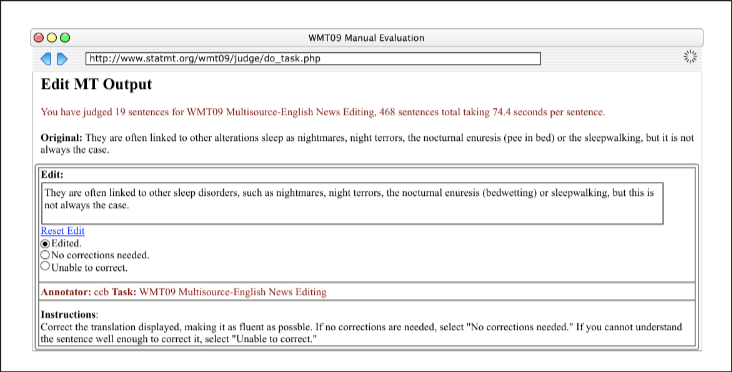
\includegraphics[width=\textwidth]{figures/edit_output.png}
        \caption{Interface for Editing MT Output}\label{fig:mt_edit}
    \end{figure}
\end{frame}


\begin{frame}{Task 3 --- Judging Acceptability}

\begin{block}{Validation of the Edits}
\begin{itemize}
    \item The Setup: A second group of judges reviews the edited sentences alongside the original reference.
    \item The Question: Is this edited version a "fully fluent and meaning-equivalent" alternative to the reference?
\end{itemize}
\end{block}

\vfill

\begin{block}{Outcome}
A simple Yes/No indicator for over 31,000 edited items.
\end{block}

\end{frame}

\begin{frame}{Task 3 --- Judging Acceptability}
    \begin{figure}[htbp]
        \centering
        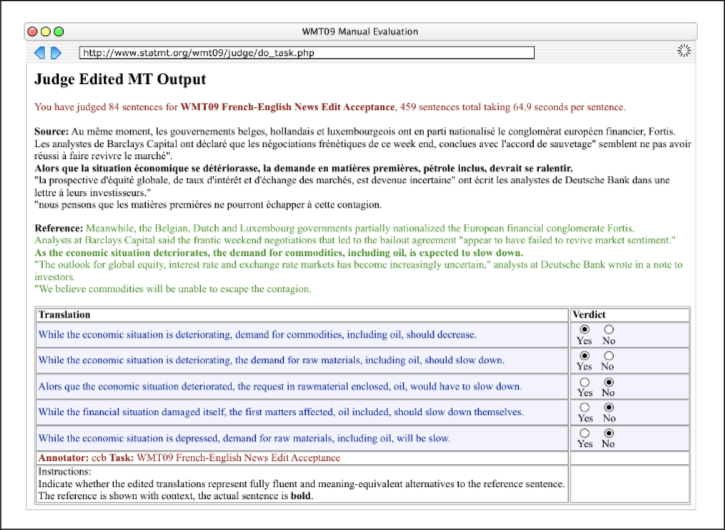
\includegraphics[width=0.75\textwidth]{figures/judge_edited_output.png}
        \caption{Interface for Editing MT Output}\label{fig:mt_edit}
    \end{figure}
\end{frame}



\begin{frame}{Quality Control – Annotator Agreement}

\begin{block}{Measuring Reliability (Kappa Coefficient K)}
\[
K = (P(A)-P(E))(1-P(E))
\]

\begin{itemize}
    \item P(A) - the proportion of times that the annotators agree
    \item P(E) - the proportion of time that they would agree by chance.
\end{itemize}

\end{block}

\vfill

\begin{itemize}
    \item Intra-annotator agreement: How often a judge agrees with themselves (Substantial: K = 0.56 – 0.73).
    \item Inter-annotator agreement: How often different judges agree (Fair/Moderate: K = 0.32 – 0.54).
\end{itemize}

\vfill

\begin{block}{Optimization}
The study found that removing the 33 worst annotators (those with the lowest agreement) improved overall data reliability while retaining 60\% of the judgments
\end{block}

\end{frame}

\begin{frame}{Task 3 --- Judging Acceptability}

\begin{figure}[t]
    \centering
    \raisebox{-0.5\height}{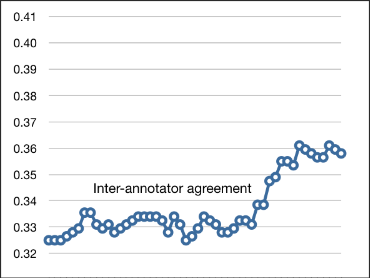
\includegraphics[width=0.3\textwidth]{figures/first50_inter_annotator.png}}
    \raisebox{-0.5\height}{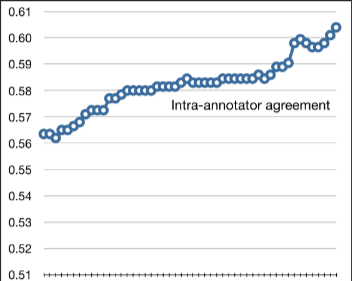
\includegraphics[width=0.3\textwidth]{figures/first50_intra_annotator.png}}
    \raisebox{-0.5\height}{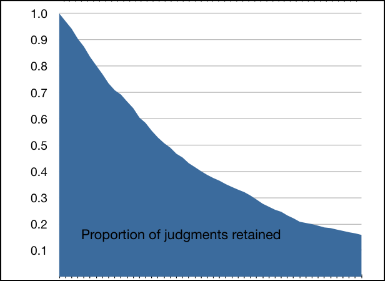
\includegraphics[width=0.3\textwidth]{figures/first50_judgements_retained.png}}
    \caption{Dropping the first 50 scores from each evaluator.}
\end{figure}
\begin{figure}[t]
    \centering
    \raisebox{-0.5\height}{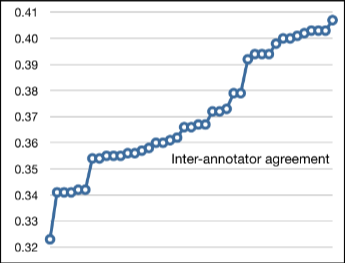
\includegraphics[width=0.3\textwidth]{figures/worst40_inter_annotator.png}}
    \raisebox{-0.5\height}{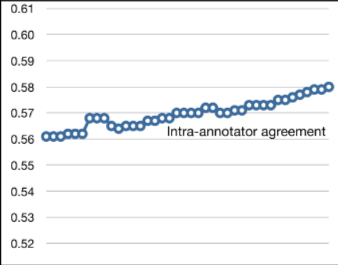
\includegraphics[width=0.3\textwidth]{figures/worst40_intra_annotator.png}}
    \raisebox{-0.5\height}{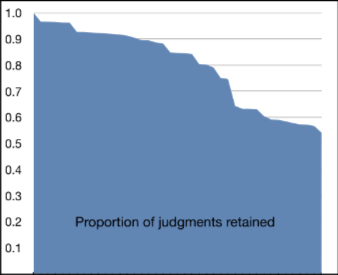
\includegraphics[width=0.3\textwidth]{figures/worst40_judgements_retained.png}}
        \caption{Dropping the worst 40 evaluators.}
\end{figure}

\end{frame}

\begin{frame}{Key Takeaways}

\begin{itemize}
    \item Human-Centric: WMT09 prioritizes human ranking over BLEU scores to validate systems.
    \item Scale: Massive crowdsourced effort from participants, volunteers, and paid staff.
    \item Innovation: Introduced "editing-based" evaluation to move beyond simple ranking.
    \item Transparency: All human judgments are made publicly available for future research.
\end{itemize}

\end{frame}
